{\color{black}
\section{Framework Resources Quantification Model}\label{model}

In this section, we introduce \textit{Framework Resources Quantification} (FRQ) model to evaluate the performance of DAG frameworks.
% The FRQ model quantifies computing and I/O resources and visualizes them in the time dimension.
The FRQ model is able to predict the execution time required by the application under most circumstances, including different DAG frameworks, hardware environments, etc.
% The FRQ model assist us in analyzing the resource scheduling of DAG framework and evaluate their performance.
We first introduce the FRQ model in Subsection \ref{model_overview}. In Subsection \ref{model_analysis}, we use the FRQ model to describe different computation jobs and discuss their performance.
% In the last Subsection \ref{model_evaluation}, we use the actual experimental results to evaluate the FRQ model.

\subsection{The FRQ Model}\label{model_overview}
% The current distributed computing frameworks mostly use DAGs to describe the computation logic. 
% A shuffle phase is required between each adjacent DAG computation phases.
{\color{black}
We propose the FRQ model to better analyze the relationship between the computation phase and the shuffle phase in the DAG computing.
% The FRQ model focuses on describing the overhead caused by the shuffle process.
The FRQ model focuses on describing the shuffle overhead which is significantly affected by the scheduling strategy.
% This overhead does not only depends on the input data size, computation speed, complexity of algorithms, and other parameters but also on which scheduling strategy the job takes.
% By using the FRQ model, we can analyze the advantages of each strategy in various situations.
After quantifying computing and I/O resources, we use the FRQ model to evaluate different resource scheduling strategies.
% For convenience, we introduce the FRQ model by taking a simple MapReduce job as an example in this section.

% Figure \ref{fig:model_basic} shows how the FRQ model describes a MapReduce job. 
As Figure \ref{fig:model_basic} shows, the FRQ model divides the job into three phases: map, shuffle, and reduce.
The horizontal axis represents time and the vertical axis represents different phases.
% As shown in Figure \ref{fig:model_basic}, the FRQ model introduce five parameters:
Firstly, we introduce five input parameters of the FRQ model:
}
\begin{itemize}
	\item Input Data Size \((D)\): The  Input data size of the job.
	\item Data Conversion Rate \((R)\): The conversion rate of the input data to the shuffle data during a computation phase.
	% This rate depends on the algorithm used in the computation phase.
    \item Computation Round Number \((N)\): The number of rounds needed to complete the computation phase. These rounds depend on the current computation resources and the configuration of the framework. Take Hadoop MapReduce as an example. Suppose we have a cluster with 50 CPUs and enough memory, the map phase consists of 200 map tasks, and each map requires 1 CPU. Then we need 4 rounds of computation to complete the map phase.
    \item Computation Speed \((V_{i})\): 
	The computation speed for each computation phase.
	% This speed depends on the algorithm used in the computation phase.
    \item Shuffle Speed \((V_{Shuffle})\): 
	Transmission speed in the shuffle phase.
	% This speed depends on network and storage device bandwidth.
\end{itemize}

\begin{figure}
    \centering
	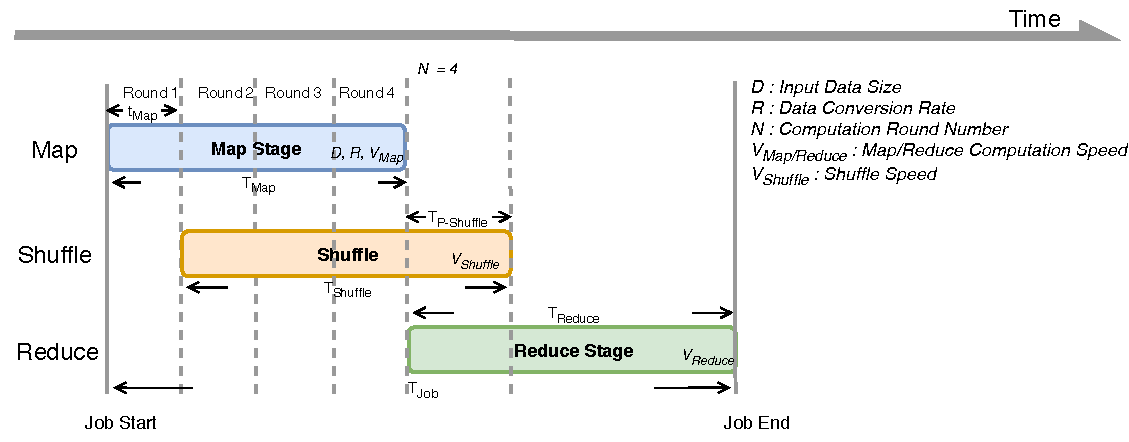
\includegraphics[width=\linewidth]{fig/model_basic}
	\caption{\color{black}Framework Resources Quantification Model\newline with Full Parallel MapReduce (\(V_{Map} \times R > V_{Shuffle}\))}
    \label{fig:model_basic}
    % \vspace{-1em}
\end{figure}
\begin{figure}
	\centering
	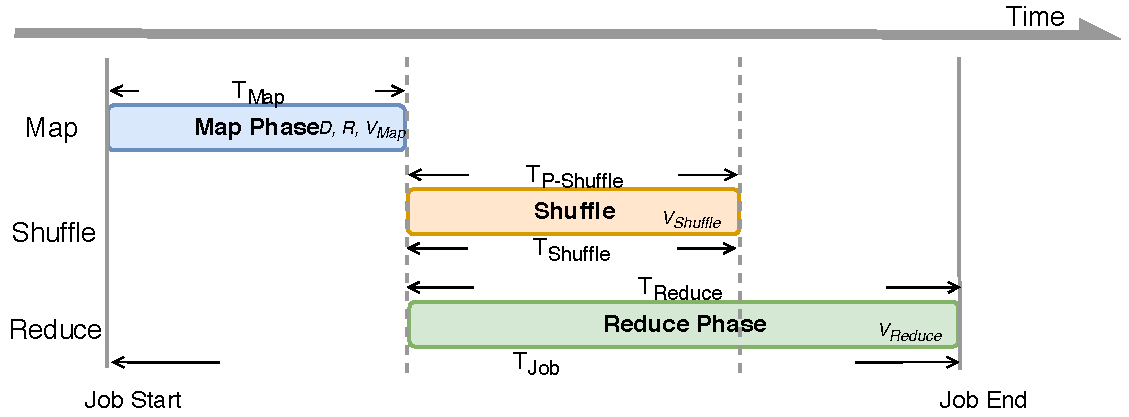
\includegraphics[width=\linewidth]{fig/model_hadoop}
	\caption{\color{black}Framework Resources Quantification Model with Half Parallel MapReduce}
	\label{fig:model_hadoop}
\end{figure}

% The FRQ model uses these overlaps to describe different scheduling strategies.
{\color{black}
Besides, the FRQ model also needs to input the scheduling strategies the framework takes.
The FRQ model needs to know the start time of each \edited{phase}.
For example, as shown in Figure \ref{fig:model_hadoop}, this strategy starts the shuffle phase and the reduce phase at the same time.
And Figure \ref{fig:model_basic} shows the pre-fetching strategy used by SCache. In the pre-fetching strategy, the shuffle phase starts as soon as it can in the map phase.
}

The FRQ model calculates the execution time of each phase of the job with these five parameters.
% As shown in Figure \ref{fig:model_basic}
The total execution time of a job is the sum of the map phase time and reduce phase time:
% \(T_{Job}=T_{Map}+T_{Reduce}\).
\begin{equation}
\label{equation_Tjob}
\begin{aligned}
    T_{Job} &= T_{Map} + T_{Reduce} + \edited{T_{Penalty}}
\end{aligned}
\end{equation}

The formulas of map phase time and shuffle phase time are as follows:
% \(T_{Map}={{\frac{D}{V_{Map}}}}\).
\begin{equation}
\label{equation_Tmap}
\begin{aligned}
    T_{Map} &= {{\frac{D}{V_{Map}}}}
\end{aligned}
\begin{aligned}
    T_{Shuffle} &= {{\frac{D}{V_{Shuffle}}}}
\end{aligned}
\end{equation}

The reduce phase time formula is as follows:
% \(T_{Reduce}=\frac{D \times R}{V_{Reduce}}+K\times T_{P\_Shuffle}\).
\begin{equation}
\label{equation_Treduce}
\begin{aligned}
    T_{Reduce} &= \frac{D \times R}{V_{Reduce}} + K \times T_{P\_Shuffle}
\end{aligned}
\end{equation}

% The shuffle phase time formula is as follows:
% \begin{equation}
% \label{equation_Tshuffle}
% \begin{aligned}
%     T_{Shuffle} &= {{\frac{D}{V_{Shuffle}}}}
% \end{aligned}
% \end{equation}

{\color{black}
\(\frac{D \times R}{V_{Reduce}}\) represents the ideal computation time of a reduce phase, and (\(K \times T_{P\_Shuffle}\)) represents the computing overhead.
\(T_{P\_Shuffle}\) represents the overlap time between the shuffle phase and the reduce phase as shown in Figure \ref{fig:model_basic}. \(T_{Shuffle}\) represents the total time of the shuffle phase. 
% The relationship between \(T_{P\_Shuffle}\) and \(T_{Shuffle}\) is determined by the resources scheduling strategy of DAG frameworks. This relationship will be shown in the following Subsection \ref{model_analysis}.  
\(K\) is an empirical value which represents the overhead caused by shuffle waiting. 
Because the computation of the reduce phase relies on the \edited{results of data transferring} of the shuffle phase, a portion of the computation needs to wait for the \edited{results of transferring}. This waiting causes the overhead.

According to Equation \ref{equation_Tjob}\&\ref{equation_Treduce}, we can optimize the job completion time by reducing \(T_{P\_Shuffle}\).
By using different resource scheduling strategies, the formulas of \(T_{P\_Shuffle}\) are different.
In the next subsection, we show the formulas and discuss the performance of different strategies.
% Improving I/O speed is an effective way to reduce shuffle time. Another optimization method is to use the idle I/O resources in the map phase for pre-fetching (see Figure \ref{fig:model_basic}). Both of the above methods can effectively reduce \(T_{P\_Shuffle}\). 
% By using the FRQ model to describe a MapReduce job, the users can analyze the resource scheduling strategy of the computation framework.
}	

\subsection{Different Scheduling Strategies on the FRQ Model}\label{model_analysis}

% \begin{figure}
% 	\centering
% 	\begin{subfigure}{\linewidth}
% 		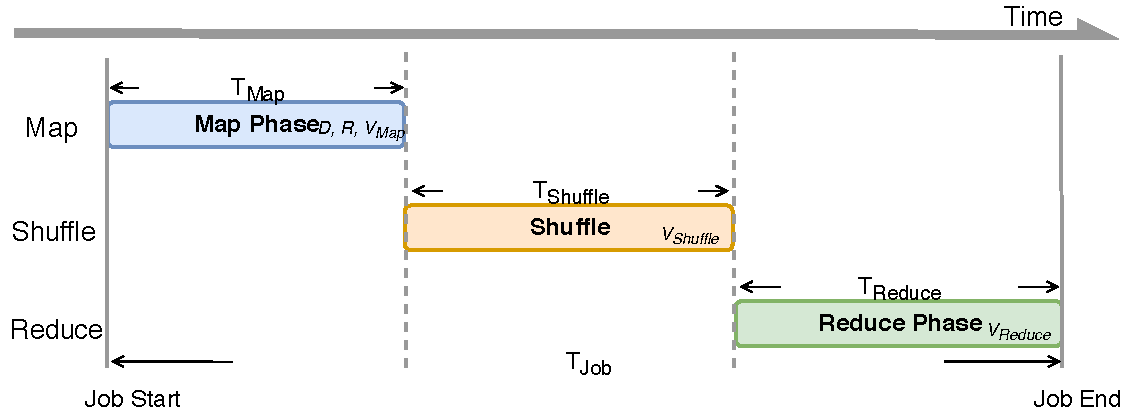
\includegraphics[width=\linewidth]{fig/model_original}
% 		\caption{\color{black}Full Serial MapReduce}
% 		\label{fig:model_original}
% 	\end{subfigure}\hfill
% 	\begin{subfigure}{\linewidth}
% 		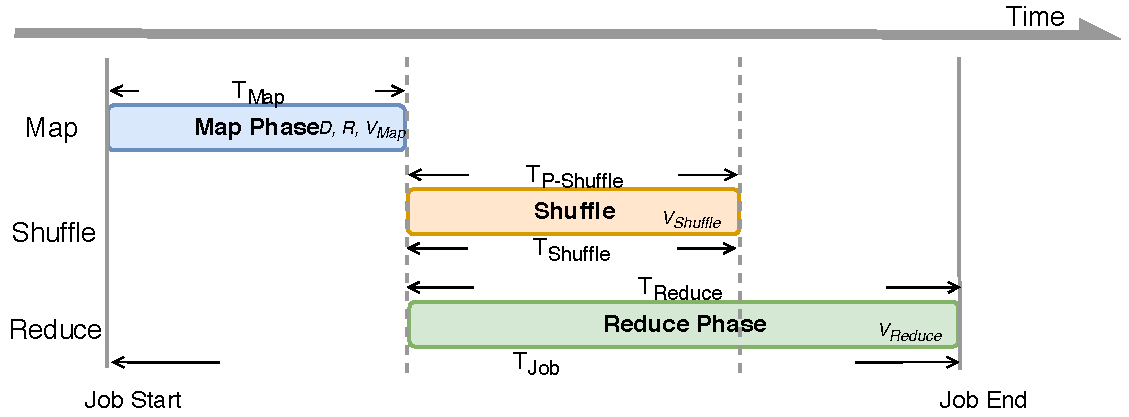
\includegraphics[width=\linewidth]{fig/model_hadoop}
% 		\caption{\color{black}Half Parallel MapReduce}
% 		\label{fig:model_hadoop}
% 	\end{subfigure}
% 	\caption{\color{black}The FRQ Model with Different Scheduling Strategies}
% 	\label{fig:model_strategies}
% \end{figure}

% The FRQ model can describe a variety of resource scheduling strategies. First, we analyze a simple scheduling strategy which used by Apache Spark by default. 
% As shown in Figure \ref{fig:model_original}, the FRQ model describes a MapReduce job that is entirely serially executed. The overlap time between the shuffle phase and the reduce phase is \(0\), in which case \(T_{P\_Shuffle}\) is \(0\). Therefore, the overhead of the reduce phase is 0. The total execution time of a job is also different from the above:
% \begin{equation}
% \label{equation_Tjob2}
% \begin{aligned}
%     T_{Job} &= T_{Map} + T_{Shuffle} + T_{Reduce}
% \end{aligned}
% \end{equation}

% Due to serialization, the I/O resource is idle during the reduce phase and map phase. This scheduling strategy is simple and has much room for optimization.

Figure \ref{fig:model_hadoop} shows a scheduling strategy which is used by Hadoop MapReduce. In this scheduling strategy, shuffle phase and reduce phase start at the same time. In this case, \(T_{P\_Shuffle}\) is equal to \(T_{Shuffle}\). Due to the increase in \(T_{P\_Shuffle}\), the time of reduce phase increases (according to Equation \ref{equation_Treduce}). Because the shuffle phase and the computation phase are executed in parallel, the total execution time of a job is the sum of \(T_{Map}\) and \(T_{Reduce}\) (see Equation \ref{equation_Tjob}). The execution time of the shuffle phase is hidden in the reduce phase. 
% However, we also found that the I/O resource in the map phase is still idle. This scheduling strategy can still be optimized.

% \begin{figure}
% 	\centering
% 	\begin{subfigure}{\linewidth}
% 		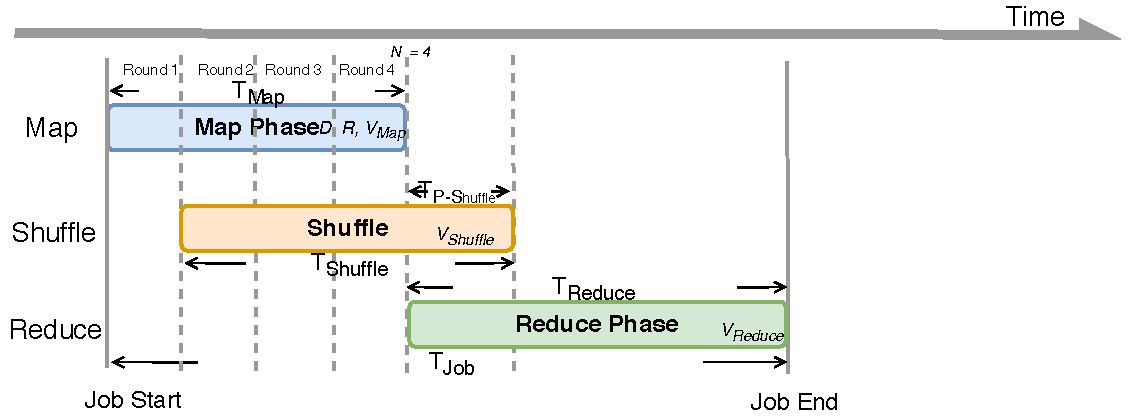
\includegraphics[width=\linewidth]{fig/model_scache1}
% 		\caption{\color{black}If \(V_{Map} \times R \ge V_{Shuffle}\)}
% 		\label{fig:model_scache1}
% 	\end{subfigure}
% 	\begin{subfigure}{\linewidth}
% 		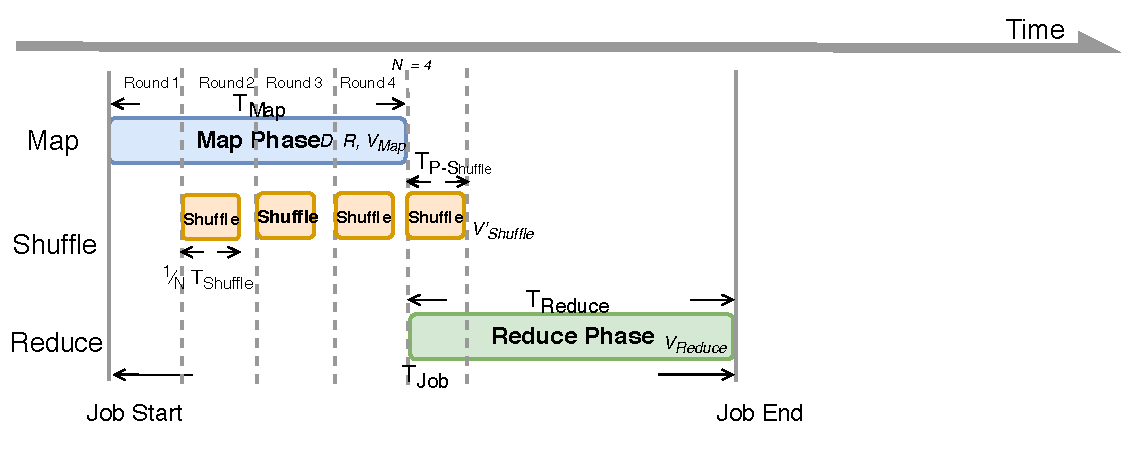
\includegraphics[width=\linewidth]{fig/model_scache2}
% 		\caption{\color{black}If \(V_{Map} \times R < V_{Shuffle}\)}
% 		\label{fig:model_scache2}
% 	\end{subfigure}
% 	\caption{\color{black}The FRQ Model with Full Parallel MapReduce in Different Environments}
% 	\label{fig:model_scache}
% \end{figure}
\begin{figure}
	\centering
	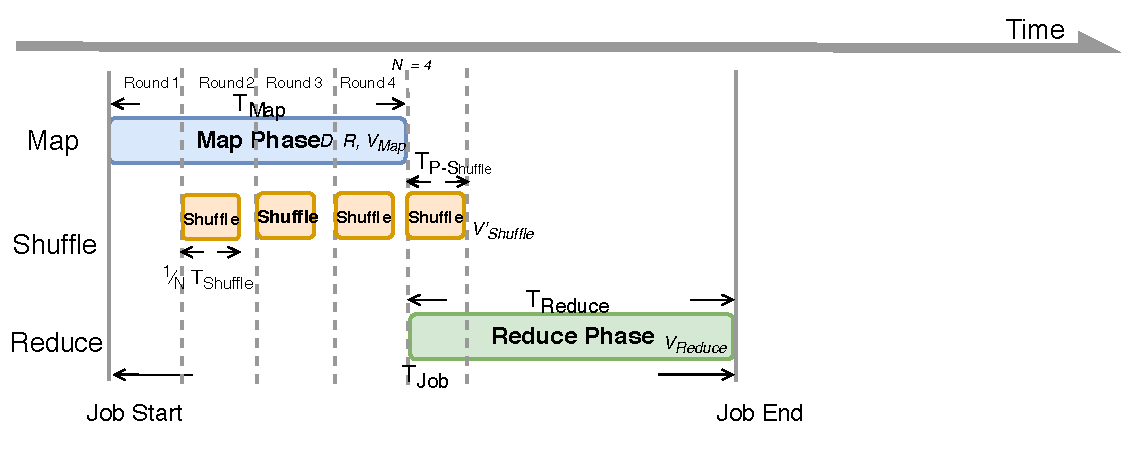
\includegraphics[width=\linewidth]{fig/model_scache2}
	\caption{\color{black}Framework Resources Quantification Model\newline with Full Parallel MapReduce (\(V_{Map} \times R < V_{Shuffle}\))}
	\label{fig:model_scache2}
\end{figure}

% Hadoop MapReduce overlaps shuffle phase with reduce phase and utilizes idle resources. We intuitively think that we can also overlap the shuffle phase and the map phases. We implemented this idea with SCache.
Figure \ref{fig:model_basic} and Figure \ref{fig:model_scache2} show the scheduling strategy for Hadoop MapReduce with SCache (Suppose N is 4).
SCache also overlaps the shuffle phase and the map phases by starting pre-fetching and pre-scheduling in the map phase.
This scheduling strategy avoids the I/O resource being idle in the map phase.
According to the design of SCache pre-fetching, we found that using the FRQ model to describe the scheduling strategy of SCache needs to distinguish two situations:

\begin{enumerate}
    \item \(V_{Map} \times R \ge V_{Shuffle}\) (Figure \ref{fig:model_basic})
	 
	The meaning of the inequality is that the speed of generating shuffle data (\(V_{Map} \times R\)) is greater than or equal to the shuffle speed (\(V_{Shuffle}\)). 
	In this situation, the shuffle phase is uninterrupted. The I/O resource will be fully utilized during the whole shuffle phase. As a result, the formula of \(T_{P\_Shuffle}\) is as followed:
	\begin{equation}
		\label{equation_Tpshuffle1}
		\begin{aligned}
			T_{P\_Shuffle} &= T_{Shuffle} - \frac{(N - 1)\times T_{Map}}{N}
		\end{aligned}
	\end{equation}
	
    \item \(V_{Map} \times R < V_{Shuffle}\) (Figure \ref{fig:model_scache2})
 
	When the shuffle speed (\(V_{Shuffle}\)) is faster, SCache needs to wait for shuffle data to be generated. As Figure \ref{fig:model_scache2} \edited{shows}, the shuffle phase will be interrupted in each round. In this case, the formula of \(T_{P\_Shuffle}\) is as followed:
	\begin{equation}
		\label{equation_Tpshuffle2}
		\begin{aligned}
			T_{P\_Shuffle} &= T_{Shuffle} \times \frac{1}{N}
		\end{aligned}
	\end{equation}
\end{enumerate}

Compared to the original Hadoop MapReduce resource scheduling strategy, Hadoop MapReduce with SCache shortens \(T_{P\_Shuffle}\) and thus shortens \(T_{Reduce}\). This is how pre-fetching optimizes the total execution time of a job.
